
\paragraph{Buff} 
Spells specialized for aiding and empowering others. \\


\subparagraph{Level 0} 
Common spells \\
\begin{tabular}{ m{2cm}m{3cm}m{4cm}m{6cm} } \hline
	\includegraphics[width=2cm]{../Pictures/Gameplay/Spells/Icon/Revelio_minima_spell_icon.jpg} & \textbf{Revelio minima} & Reveals secrets about a person or object. Your magic grants you a brief insight into the target's defenses. & On your next turn, you gain advantage on your first attack roll against the target, provided that this spell hasn't ended. \\ \hline
   
\includegraphics[width=2cm]{../Pictures/Gameplay/Spells/Icon/Inveterasco_spell_icon.png} & \textbf{Inveterasco} & Helps the caster focus better on his current task & Once before the spell ends, the target of the spell can roll a d4 and add the number rolled to one ability check of its choice. The spell then ends. \\ \hline
\end{tabular}

\subparagraph{Level 1} 
Low level spells \\
\begin{tabular}{ m{2cm}m{3cm}m{4cm}m{6cm} } \hline
	
\includegraphics[width=2cm]{../Pictures/Gameplay/Spells/Icon/Empowering_spell_icon.png} & \textbf{Empowering Charm} & Invigorates the spirits of the targets of this spell. & You choose up to three creatures of your choice within range. Whenever a target makes an attack roll or a saving throw before the spell ends, the target can roll a d4 and add the number rolled to the attack roll or saving throw. \\ \hline

\includegraphics[width=2cm]{../Pictures/Gameplay/Spells/Icon/Engorgio_spell_icon.png} & \textbf{Engorgio / Reducio} & Causes the target to swell or dwindle in physical size. & \textbf{Enlarged}: dimensions doubled, adv. in STR checks and saving throws, +1d4 to target weapons. \textbf{Reduced}: dimensions halved, disadv. in STR checks and saving throws, -1d4 to target weapons (can't be less than 1).  \\ \hline
\end{tabular}

\subparagraph{Level 3} 
Medium spells \\
\begin{tabular}{ m{2cm}m{3cm}m{4cm}m{6cm} } \hline
	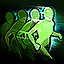
\includegraphics[width=2cm]{../Pictures/Gameplay/Spells/Icon/Haste_spell_icon.png} & \textbf{Quickening Charm} & Makes a target hasten its movements and thoughts. & Choose a willing creature that you can see within range. Until the spell ends, the target's speed is doubled, it gains a +2 bonus to AC, it has advantage on Dexterity saving throws, and it gains an additional action on each of its turns. \\ \hline
   
\includegraphics[width=2cm]{../Pictures/Gameplay/Spells/Icon/Heroism_spell_icon.png} & \textbf{Power of Belief } & Imbues the target of the spell with unprecedented bravery & Until the spell ends, up to three creatures are immune to being frightened and gain temporary hit points equal to your spellcasting ability modifier at the start of each of its turns. When the spell ends, the targets lose any remaining temporary hit points from this spell. At Higher Levels: When you cast this spell using a spell slot of 2nd level or higher, you can target one additional creature for each slot level above 1st. \\  \hline
\end{tabular}

\subparagraph{Level 5} 
Greater spells \\
\begin{tabular}{ m{2cm}m{3cm}m{4cm}m{6cm} } \hline
	
\includegraphics[width=2cm]{../Pictures/Gameplay/Spells/Icon/Salvio_Hexia_spell_icon.png} & \textbf{Salvio Hexia} & Makes an area magically secure, protecting against hexes and spells. &  The spell prevents any physical or magical method from seeing what's inside of the secured area from the outside. At Higher Levels. When you cast this spell using a spell slot of 5th level or higher, you can increase the size of the cube by 100 feet for each slot level beyond 4th. Thus you could protect a cube that can be up to 200 feet on one side by using a spell slot of 5th level.\\ \hline
\end{tabular}

\subparagraph{Level 7} 
Superior spells \\
\begin{tabular}{ m{2cm}m{3cm}m{4cm}m{6cm} } \hline
	
\includegraphics[width=2cm]{../Pictures/Gameplay/Spells/Icon/Occlumency_spell_icon.png} & \textbf{Occlumency} & Prevents legilimency and other harming effects on the mind. & Until the spell ends, one willing creature you touch is immune to psychic damage, any effect that would sense its emotions or read its thoughts, divination spells, and the charmed condition. \\ \hline
\end{tabular}

\subparagraph{Level 8} 
Supreme spells \\
\begin{tabular}{ m{2cm}m{3cm}m{4cm}m{6cm} } \hline
	\includegraphics[width=2cm]{../Pictures/Gameplay/Spells/Icon/Righteous_aura_spell_icon.png} & \textbf{Righteous aura} & Invigorating light washes out around the caster. & Each creature chosen by the caster around him has advantage on all saving throws and other creatures has disavantage on attack rolls on them. The attacker must succeed on a CON saving throw or be blinded for 1 turn. \\ \hline
\end{tabular}

\pagebreak













